\documentclass[12pt]{article}

\usepackage[a4paper, left=3.17cm, right=3.17cm, top=2.54cm, bottom=2.54cm]{geometry}
\usepackage[T1]{fontenc}
\usepackage{mathptmx}
\usepackage{amsmath}
\usepackage{amsfonts}
\usepackage{chemformula}
\usepackage{cite}
\usepackage[colorlinks, linkcolor=black, anchorcolor=black, citecolor=black]{hyperref}
\usepackage{graphicx}
\usepackage{fancyhdr}
\usepackage{enumitem}
\usepackage{listings}
\usepackage{setspace}
\usepackage[a4paper]{geometry}
\usepackage[ruled]{algorithm2e}

\geometry{left=2.2cm, right=2.2cm, top=3cm, bottom=2.5cm}

\setlength{\parskip}{0.5em}
\title{Skip List \\ \bigskip \large Project7\ \ Report\ \ by\ \ Group1}
\author{Wu Yihang \\ Sun Xinjie \\ Guo Jiahao}

\lstset{
    columns=fixed,       
    numbers=left,                                        % 在左侧显示行号
    numberstyle=\tiny\color{gray},                       % 设定行号格式
    frame=none,                                          % 不显示背景边框
    backgroundcolor=\color[RGB]{245,245,244},            % 设定背景颜色
    keywordstyle=\color[RGB]{40,40,255},                 % 设定关键字颜色
    numberstyle=\tiny,keywordstyle=\color{blue!70},
    commentstyle=\color{red!50!green!50!blue!50},frame=shadowbox,
    rulesepcolor=\color{red!20!green!20!blue!20},basicstyle=\ttfamily,
    stringstyle=\rmfamily\slshape\color[RGB]{128,0,0},   % 设置字符串格式
    showstringspaces=false,                              % 不显示字符串中的空格
    language=C++,                                        % 设置语言
    }

\pagestyle{fancy}
\fancyhf{}
\cfoot{\thepage}
\fancyhead[C]{Advanced Data Structure and Algorithm Analysis\ \ \ \ Project7  Report\ \ \ \ Group1}
\begin{document}

\begin{titlepage}
	\newcommand{\HRule}{\rule{\linewidth}{0.5mm}}
	\begin{figure}
        \flushleft
        
\includegraphics[scale=0.4]{0.png}
    \end{figure}
    \center 
	\quad\\[1.5cm]
	\textsl{\Large Zhejiang University }\\[0.5cm] 
	\textsl{\large College of Computer Science and Technology}\\[0.5cm] 
	\makeatletter
	\HRule \\[0.4cm]
	{ \huge \bfseries \@title}\\[0.4cm] 
	\HRule \\[1.5cm]
	\begin{minipage}{0.4\textwidth}
		\begin{flushleft} \Large
			\emph{Author:}\\
			\@author 
		\end{flushleft}
	\end{minipage}
	~
	\begin{minipage}{0.4\textwidth}
		\begin{flushright} \Large
			\emph{Supervisor:} \\
			\textup{Mao Yuchen}
		\end{flushright}
	\end{minipage}\\[2cm]
	\makeatother
	\begin{flushleft}
        \Large
        \textbf{Abstract:}

        \large{In this project, we implement a probabilisitc data structure that is built upon the general idea of a linked list
        named skip list. We not only ensure the correctness of our implementation for searching, inserting and deleting, 
        but analyze the the time complexity, which is $O(\textup{log}n)$, of these operations theoretically based on 
        probability theory and pratically based on experiments on inputs of different size.}
    \end{flushleft}
    
    {\large An Assignment submitted for the ZJU:}\\[0.5cm]
	{\large {21120491\ \ Advanced Data Structure and Algorithm Analysis}}\\[0.5cm]
	{\large \today}\\[2cm] 
	\vfill 
\end{titlepage}
    
    \section{Introduction of the Project}
    In this project, we need to implement a probabilisitc data structure that 
    is built upon the general idea of a linked list named skip list.
    We need to implement three basic operations: searching, inserting, 
    and deleting. Except that, we need to analyze these operations not 
    only theoretically but also pratically. We need to measure the practical 
    performance of skip list on inputs of different size.

    \section{Introduction to the Skip List}
    \subsection{Structure Property}
    Fibonacci heap is a data structure for priority queue operations, 
    which is is a collection of trees satisfying the minimum-heap property, that is, the key 
    of a child is always greater than or equal to the key of the parent.
    \begin{figure}[h]
        \centering
        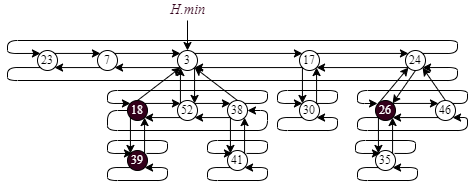
\includegraphics[scale=0.7]{heap.png}
        \caption{An example of a Fibonacci heap}
    \end{figure}

    As Figure 1 shows, we access a given Fibonacci heap H by a pointer \textbf{H.min} to the root of a tree
    containing the minimum key. When a Fibonacci heap H is empty, H.min
    is NULL. The roots of all the trees in a Fibonacci heap are linked together using their
    \textbf{left} and \textbf{right} pointers into a circular, doubly linked list called \textbf{root list}.
    
    We also see that each node x contains a pointer \textbf{x.p} to its parent and
    a pointer \textbf{x.child} to any one of its children. Each child y of x are linked together
    in a circular, doubly linked list, which we call the \textbf{child list of x}, using pointers 
    \textbf{y.left} and \textbf{y.right} that point to y’s left and right siblings. 
    If node y is an only child, then y.left=y.right=y. Siblings may
    appear in a child list in any order.
    
    Except that, other property we need for the node are:
    \begin{enumerate}
        \setlength{\itemsep}{0pt}
        \item \textbf{x.degree}: store the number of children in the child
        list of node x.
        \item \textbf{x.mark}: indicates whether node x has lost a child 
        since the last time x was made the child of another node.
    \end{enumerate}

    We also need \textbf{H.n} as a heap attribute, which represent the number of nodes currently in H.
    \subsection{Implementation of Operations}
    \subsubsection{Insertion}
    Insertion for Fibonacci heap is a lazy operation. The following procedure inserts node \emph{x} into Fibonacci heap \emph{H}:
    \begin{algorithm}
        \caption{Insertion for Fibonacci heap}
        \LinesNumbered
        \KwIn{Fibonacci heap \emph{H}, node \emph{x}}
        \emph{x.degree} = 0\;
        \emph{x.p} = \emph{x.child} = NULL\;
        \emph{x.mark} = false\;
        \eIf{H.min == \textup{NULL}}{
            create a root list for \emph{H} containing just \emph{x}\;
            \emph{H.min} = \emph{x}\;
        }{
            insert \emph{x} into \emph{H}'s root list\;
            \If{x.key < H.min.key}{
                \emph{H.min = x}\;
            }
        }
        \emph{H.n} = \emph{H.n} + 1
    \end{algorithm}

    First we initialize some attributes of node \emph{x}. Next, we test if Fibonacci heap \emph{H} is empty. 
    If it is, we make \emph{x} be the only node in \emph{H}’s root list and set \emph{H.min} to point to \emph{x}. 
    Otherwise, we insert \emph{x} into \emph{H}’s root list and update \emph{H.min} if necessary. Finally, we increment \emph{H.n}.

    \subsubsection{Make heap}
    For the making heap operation of Fibonacci heap, we just need 
    to insert n keys continuously.

    \subsubsection{FindMin}
    Because we maintain a pointer to the minimum node of the heap, 
    so we only need to return \emph{H.min.data}.
    \subsubsection{DeleteMin}
    DeleteMin is much more complicated than insertion. It works by first making a root
    out of each of the minimum node’s children and removing the minimum node from
    the root list. It then consolidate the root list by linking roots of equal degree until
    at most one root remains of each degree. The pseudocode of Algorithm 2 extracts the minimum node.
    
    The procedure consolidate uses an auxiliary array \emph{A}, whose size can be limited by the bounding the maximum degree
    $$D(n) \le \lfloor\log_{\phi}n\rfloor,\quad \phi = (1 + \sqrt{5}) / 2$$
    , to keep track of roots according to their degrees. If \emph{A}[\emph{i}] = \emph{y}, then \emph{y} is currently a root
    with \emph{y.degree = i}.

    In detail, let's see the pseudocode of Algorithm 3, the consolidate procedure works as follows. 
    We first allocate array \emph{A}, then we link roots together, \emph{w} may be linked
    to some other node and no longer be a root. Nevertheless, \emph{w} is always in a tree
    rooted at some node \emph{x}, which may or may not be \emph{w} itself. Because we want at
    most one root with each degree, we look in the array \emph{A} to see whether it contains
    a root \emph{y} with the same degree as \emph{x}. If it does, then we link the roots \emph{x} and \emph{y} but
    guaranteeing that \emph{x} remains a root after linking. That is, we link \emph{y} to \emph{x} after first
    exchanging the pointers to the two roots if \emph{y}’s key is smaller than \emph{x}’s key. After
    we link \emph{y} to \emph{x}, the degree of \emph{x} has increased by 1, and so we continue this process,
    linking \emph{x} and another root whose degree equals \emph{x}’s new degree, until no other root
    that we have processed has the same degree as \emph{x}. We then set the appropriate entry
    of \emph{A} to point to \emph{x}, so that as we process roots later on, we have recorded that \emph{x} is
    the unique root of its degree that we have already processed. When this for loop
    terminates, at most one root of each degree will remain, and the array \emph{A} will point
    to each remaining root.

    \begin{algorithm}
        \caption{DeleteMin for Fibonacci heap}
        \LinesNumbered
        \KwIn{Fibonacci heap \emph{H}}
        \emph{z = H.min}\;
        \If{z \textup{!= NULL}}{
            \For{\textup{each child} x \textup{of} z}{
                add \emph{x} to the root list of \emph{H}\;
                \emph{x.p = }NULL
            }
            remove \emph{z} from the root list of \emph{H}\;
        \eIf{z == z.right}{
            \emph{H.min} = NULL\;
        }(\emph{H.min = z.right}){
            consolidate(\emph{H})\;
        }
        \emph{H.n} = \emph{H.n} - 1
        }
    \end{algorithm}

    \begin{algorithm}
        \caption{Consolidate for Fibonacci heap}
        \LinesNumbered
        \KwIn{Fibonacci heap \emph{H}, node \emph{x}}
        let \emph{A} be a new array\;
        \For{i = \textup{0 to size of} A}{
            \emph{A}[\emph{i}] = NULL\;
        }
        \For{\textup{each node} w \textup{in the root list of} H}{
            \emph{x = w}\;
            \emph{d = x.degree}\;
            \While{A\textup{[}d\textup{]} \textup{!= NULL}}{
                \emph{y = A}[\emph{d}]\;
                \If{x.key > y.key}{
                    exchange \emph{x} with \emph{y}\;
                }
                remove \emph{y} from the root list of \emph{H}\;
                make \emph{y} a child of \emph{x}, incrementing \emph{x.degree}\;
                \emph{y.mark} = false\;
                \emph{A}[\emph{d}] = NULL\;
                \emph{d = d} + 1\;
            }
            \emph{A}[\emph{d}] = \emph{x}\;
        }
        \emph{H.min} = NULL\;
        \For{i = \textup{0 to size of} A}{
            \If{A\textup{[}d\textup{] != NULL}}{
                \eIf{H.min == \textup{NULL}}{
                    create a root list for \emph{H} containing just \emph{A}[\emph{i}]\;
                    \emph{H.min} = \emph{A}[\emph{i}]\;
                }{
                    insert \emph{A}[\emph{i}] into \emph{H}'s root list\;
                    \If{A\textup{[}i\textup{]}.key < H.min.key}{
                        \emph{H.min = A}[\emph{i}]\;
                    }
                }
            }
        }
    \end{algorithm}

    \subsubsection{Merge}
    We don't need this procedure in this project, so I just describe
    this procedure without pseudocode. To merge two Fibonacci heaps $H_{1}$ and $H_{2}$, 
    we first concatenate the root lists of $H_{1}$ and $H_{2}$ into a new root list \emph{H}. 
    Then we set the minimum node of \emph{H} and new \emph{H.n}.

    \subsubsection{DecreseKey}
    DecreseKey operation is crucial for the optimization for Dijkstra's algorithm
    because it has only \emph{O}(1) amortized time. To implement the operation, 
    we first judge if the min-heap order has not been violated, if it is, we don't need to adjust the position of the node.
    If min-heap order has been violated, many changes may occur. We start by
    cutting procedure, which “cuts” the link between x and its parent y,
    making x a root.

    We use the mark attributes to obtain the desired time bounds.
    As soon as the second child has been lost, we cut \emph{x} from its parent, making it a new
    root, and sometimes we need cascading-cut operation. Once all the cascading 
    cuts have occurred, the procedure can finish up by updating \emph{H.min} if necessary. The only node whose key changed
    was the node \emph{x} whose key decreased. Thus, the new minimum node is either the
    original minimum node or node \emph{x}.

    \begin{algorithm}
        \caption{DecreseKey for Fibonacci heap}
        \LinesNumbered
        \KwIn{Fibonacci heap \emph{H}, node \emph{x}, new key value \emph{k}}
        \If{k > x.key}{
            \textbf{error}"new key is greater than current key"\;
        }
        \emph{x.key = k}\;
        \emph{y = x.p}\;
        \If{y\textup{!= NULL and }x.key < y.key}{
            remove \emph{x} from the child list of \emph{y}, decrementing \emph{y.degree}\;
            add \emph{x} to the root list of \emph{H}\;
            \emph{x.p} = NULL\;
            \emph{x.mark} = false\;
            cascading\_cut(\emph{H}, \emph{y})\;
        }
        \If{x.key < H.min.key}{
            H.min = x\;
        }
    \end{algorithm}

    \begin{algorithm}
        \caption{Cascade cut for Fibonacci heap}
        \LinesNumbered
        \KwIn{Fibonacci heap \emph{H}, node \emph{y}}
        \emph{z = y.p}\;
        \If{z\textup{!= NULL}}{
            \eIf{y.mark == \textup{false}}{
                \emph{y.mark} = true\;
            }{
                remove \emph{y} from the child list of \emph{z}, decrementing \emph{z.degree}\;
                add \emph{y} to the root list of \emph{H}\;
                \emph{y.p} = NULL\;
                \emph{y.mark} = false\;
                cascading\_cut(\emph{H}, \emph{z})\;
            }
        }
    \end{algorithm}
    \subsubsection{Delete}
    For deletion, we just need to use decrease key function to decrease
    the data stored in the node we want to delete to a small value that 
    normal node won't store. 

    \section{Theoretical Analysis}
    \subsection{Heap Operations}
    In this section, we define n as the number of elements in 
    priority queue. And the result in the table represent the 
    worst time, \textbf{except the column for Fibonacci heap, which
    represent amortized time}. 
    \begin{table}[h]
        \centering
		\begin{tabular}{l l l l l}
			
			\textbf{Operation} & \textbf{Binary heap} & \textbf{Leftist heap} & \textbf{Binomial heap} & \textbf{Fibonacci heap}\\
			
			Make heap    & \emph{O}(\emph{n}) & \emph{O}(\emph{n}) & \emph{O}(\emph{n}) & \emph{O}(\emph{n})\\
			Find min     & \emph{O}(1)        & \emph{O}(1)        & \emph{O}(1)        & \emph{O}(1)\\
			Insert       & \emph{O}(log\emph{n}) & \emph{O}(log\emph{n}) & \emph{O}(log\emph{n}) & \emph{O}(1)\\
            Delete min   & \emph{O}(log\emph{n}) & \emph{O}(log\emph{n}) & \emph{O}(log\emph{n}) & \emph{O}(log\emph{n})\\
            Merge        & \emph{O}(\emph{n}) & \emph{O}(log\emph{n}) & \emph{O}(log\emph{n}) & \emph{O}(1)\\
            Delete       & \emph{O}(log\emph{n}) & \emph{O}(log\emph{n}) & \emph{O}(log\emph{n}) & \emph{O}(log\emph{n})\\
            Decrese key  & \emph{O}(log\emph{n}) & \emph{O}(log\emph{n}) & \emph{O}(log\emph{n}) & \emph{O}(1)
		\end{tabular}
		\caption{Running times of all operations of different heaps}
	\end{table}
    \subsection{optimization for Dijkstra's Algorithm}
    We have learned that theoretically, the total running time of 
    Dijkstra's algorithm without priority queue is $O(|E|+|V|^{2})$. 
    So if the graph is dense, with $|E| = \Theta(|V|^{2})$, the algorithm 
    without priority queue is good enough.

    But in practice, also in this project, the grapg is always sparse, 
    which means $|E| = \Theta(|V|)$, the algorithm is too slow. 
    So we consider the heap operation DeleteMin, whose running time is 
    $O(n\textup{log}n)$ in all the heaps we use in the project, to find and delete the
    minimum vertex. And we use DecreseKey, or in practice insertion, whose 
    running time is $O(n\textup{log}n)$ for binary heap, leftist heap,  
    binomial heap, and $O(1)$ for Fibonacci heap.

    The improtant observation is that the running time of Dijkstra algorithm 
    is dominated by $|E|$ DecreseKey/Insertion operation and $|V|$ DeleteMin 
    operations. So theoretically, for binary heap, leftist heap and binomial 
    heap, the time bound for the optimized Dijkstra algorithm is 
    $O(|E|\textup{log}|V| + |V|\textup{log}|V|) = O(|E|\textup{log}|V|)$, and for Fibonacci heap, 
    the time bound will be decreased to $O(|E| + |V|\textup{log}|V|)$.

    \section{Experiment and Result}
        
    \section{Discussion and Conclusion}
        
\end{document}